% 请确保文件编码为utf-8,使用XeLaTex进行编译,或者通过overleaf进行编译

\documentclass[answers]{exam}  % 使用此行带有作答模块
% \documentclass{exam} % 使用此行只显示题目

\usepackage{xeCJK}
\usepackage{zhnumber}
\usepackage{graphicx}
\usepackage{hyperref}
\usepackage{amsmath}
\usepackage{booktabs}
\usepackage{enumerate}
\usepackage{amssymb}
\usepackage{listings}
\usepackage{floatrow}
\usepackage{blindtext}
\usepackage{subcaption}
\pagestyle{headandfoot}
\firstpageheadrule
\firstpageheader{南京大学}{机器学习导论}{习题三}
\runningheader{南京大学}
{机器学习导论}
{习题二}
\runningheadrule
\firstpagefooter{}{第\thepage\ 页(共\numpages 页)}{}
\runningfooter{}{第\thepage\ 页(共\numpages 页)}{}


\setlength\linefillheight{.5in}

\renewcommand{\solutiontitle}{\noindent\textbf{解:}\par\noindent}

\renewcommand{\thequestion}{\zhnum{question}}
\renewcommand{\questionlabel}{\thequestion .}
\renewcommand{\thepartno}{\arabic{partno}}
\renewcommand{\partlabel}{\thepartno .}

\lstset{language=Matlab}%这条命令可以让LaTeX排版时将Matlab关键字突出显示
\lstset{
	breaklines,%这条命令可以让LaTeX自动将长的代码行换行排版
	basicstyle=\footnotesize\ttfamily, % Standardschrift
	backgroundcolor=\color[rgb]{0.95,0.95,0.95},
	keywordstyle=\color{blue},
	commentstyle=\color{cyan},
	tabsize=4,numbers=left,
	numberstyle=\tiny,
	frame=single,
	%numbers=left, % Ort der Zeilennummern
	numberstyle=\tiny, % Stil der Zeilennummern
	%stepnumber=2, % Abstand zwischen den Zeilennummern
	numbersep=5pt, % Abstand der Nummern zum Text
	tabsize=2, % Groesse von Tabs
	extendedchars=false, %
	breaklines=true, % Zeilen werden Umgebrochen
	keywordstyle=\color{red},%这一条命令可以解决代码跨页时, 章节标题, 页眉等汉字不显示的问题
	stringstyle=\color{white}\ttfamily, % Farbe der String
	showspaces=false, % Leerzeichen anzeigen ?
	showtabs=false, % Tabs anzeigen ?
	xleftmargin=17pt,
	framexleftmargin=17pt,
	framexrightmargin=5pt,
	framexbottommargin=4pt,
	%backgroundcolor=\color{lightgray},
	showstringspaces=false % Leerzeichen in Strings anzeigen ?
}
\renewcommand{\lstlistingname}{CODE}
\lstloadlanguages{% Check Dokumentation for further languages ...
	%[Visual]Basic
	%Pascal
	%C
	%Python
	%XML
	%HTML
	%Java
}
%%% load AMS-Latex Package
\usepackage{amssymb}
\usepackage{amsmath,amsfonts}
% \usepackage{amsthm}
\usepackage{amsopn}
\usepackage{bm} % bold symbol
\usepackage{multirow}



% operator in optimization
\DeclareMathOperator{\argmax}{arg\,max}
\DeclareMathOperator{\argmin}{arg\,min}
\DeclareMathOperator{\softmax}{softmax}

% special functions
\newcommand{\trace}[1]{\operatornamewithlimits{tr}\left\{#1\right\}}
\newcommand{\diag}{\operatornamewithlimits{diag}}
\newcommand{\sign}{\operatornamewithlimits{sign}}
\newcommand{\const}{\operatornamewithlimits{const}}

% special display
\newcommand{\parde}[2]{\frac{\partial #1}{\partial  #2}}

% define vector and matrix symbols
\newcommand{\vct}[1]{\boldsymbol{#1}} % vector
\newcommand{\mat}[1]{\boldsymbol{#1}} % matrix
\newcommand{\cst}[1]{\mathsf{#1}}  % constant

% shorthand
\newcommand{\vtheta}{\vct{\theta}}
\newcommand{\vmu}{\vct{\mu}}
\newcommand{\vc}{\vct{c}}
\newcommand{\vp}{\vct{p}}
\newcommand{\vq}{\vct{q}}
\newcommand{\vx}{{\vct{x}}}
\newcommand{\vy}{\vct{y}}
\newcommand{\vz}{{\vct{z}}}
\newcommand{\vu}{\vct{u}}
\newcommand{\vo}{{\vct{o}}}
\newcommand{\va}{\vct{a}}
\newcommand{\vb}{\vct{b}}
\newcommand{\ve}{\vct{e}}
\newcommand{\vr}{\vct{r}}
\newcommand{\vt}{\vct{t}}
%\newcommand{\vpsi}{\vct{\psi}}
\newcommand{\vs}{\vct{s}}
\newcommand{\vv}{\vct{v}}
\newcommand{\vw}{\vct{w}}
\newcommand{\vzero}{\vct{0}}
\newcommand{\vf}{\vct{f}}
\newcommand{\vh}{\vct{h}}
\newcommand{\vg}{\vct{g}}
\newcommand{\vphi}{\vct{\phi}}
\newcommand{\vpsi}{\vct{\psi}}
\newcommand{\ones}{\vct{1}}
\newcommand{\mU}{\mat{U}}
\newcommand{\mA}{\mat{A}}
\newcommand{\mB}{\mat{B}}
\newcommand{\mC}{\mat{C}}
\newcommand{\mD}{\mat{D}}
\newcommand{\mV}{\mat{V}}
\newcommand{\mW}{\mat{W}}
\newcommand{\mH}{\mat{H}}
\newcommand{\mI}{\mat{I}}
\newcommand{\mP}{\mat{P}}
\newcommand{\mS}{\mat{S}}
\newcommand{\mJ}{\mat{J}}
\newcommand{\mM}{\mat{M}}
\newcommand{\mT}{\mat{T}}
\newcommand{\mZ}{\mat{Z}}
\newcommand{\mO}{\mat{O}}
\newcommand{\mX}{\mat{X}}
\newcommand{\mY}{\mat{Y}}
\newcommand{\mQ}{\mat{Q}}
\newcommand{\mLambda}{\mat{\Lambda}}
% \newcommand{\mL}{\mat{L}}
\newcommand{\mmI}{\mat{I}}
\newcommand{\mK}{\mat{K}}
\newcommand{\mSigma}{\mat{\Sigma}}
\newcommand{\mOmega}{\mat{\Omega}}
\newcommand{\cC}{\cst{C}}
\newcommand{\cM}{\cst{M}}
\newcommand{\cN}{\cst{N}}
\newcommand{\cQ}{\cst{Q}}
\newcommand{\cD}{\cst{D}}
\newcommand{\cL}{\cst{L}}
\newcommand{\cK}{\cst{K}}
\newcommand{\cH}{\cst{H}}
\newcommand{\cR}{\cst{R}}
\newcommand{\cU}{\cst{U}}
\newcommand{\cS}{\cst{S}}
\newcommand{\cX}{\cst{X}}
\newcommand{\sQ}{\mathcal{Q}}
\newcommand{\sS}{\mathcal{S}}
\newcommand{\sF}{\mathcal{F}}
\newcommand{\sC}{\mathcal{C}}
\newcommand{\sX}{\mathcal{X}}
\newcommand{\sH}{\mathcal{H}}

\newcommand{\bE}{\mathbb{E}}
\newcommand{\bR}{\mathbb{R}}
\newcommand{\bH}{\mathbb{H}}

\usepackage{algorithm}  
% \usepackage{algorithmic}
%\usepackage{algorithmicx}  
\usepackage{algpseudocode}  

\floatname{algorithm}{算法}  
\renewcommand{\algorithmicrequire}{\textbf{输入:}}  
\renewcommand{\algorithmicensure}{\textbf{输出:}}  

\begin{document}
\Large
\noindent
% 姓名学号
姓名:麻超 \\
学号:201300066 \\
\begin{questions}
    \question [20] \textbf{利用信息熵进行决策树划分}

    \begin{enumerate}
        \item  对于不含冲突样本(即属性值相同但标记不同的样本)的训练集, 必存在与训练集一致(训练误差为0)的决策树. 如果训练集可以包含无穷多个样本, 是否一定存在与训练集一致的深度有限的决策树? 并说明理由 (仅考虑每次划分仅包含一次属性判断的决策树).
        \item
              信息熵$\operatorname{Ent}(D)$定义如下
              \begin{align}
                  \operatorname{Ent}(D)=-\sum_{k=1}^{|\mathcal{Y}|}\; p_{k} \log_{2} p_{k}\label{ch4_eq:entropy}
              \end{align}
              请证明信息熵的上下界为
              \begin{equation}
                  0 \leq \operatorname{Ent}(D)\leq \log _{2}|\mathcal{Y}|
              \end{equation}
              并给出等号成立的条件.
        \item  在ID3决策树的生成过程中, 需要计算信息增益(information gain)以生成新的结点. 设离散属性$a$有$V$个可能取值$\left\{a^{1}, a^{2}, \cdots, a^{V}\right\}$, 请考教材4.2.1节相关符号的定义证明:
              \begin{equation}
                  \operatorname{Gain}(D, a)=\operatorname{Ent}(D)-\sum_{v=1}^{V} \frac{\left|D^{v}\right|}{|D|} \operatorname{Ent}\left(D^{v}\right) \geq 0
              \end{equation}
              即信息增益非负.
    \end{enumerate}
    \begin{solution}
        \begin{enumerate}
            \item 存在.

                  已知对于不含冲突样本的训练集,存在和训练集一致的决策树,那么当决策树达到最大深度之后,每一个叶节点必然会对应唯一的一个样本或者所有属性都和标记相同的多个样本,即叶节点标记与样本自身标记相同,此时训练误差为0,也就是训练集和决策树一致.因为样本特征数量有限,所以属性数量同时决定了决策树深度最大值,故决策树深度有限.
            \item $\operatorname{Ent}(D)=f(p_1,p_2,...,p_n)=-\sum_{k=1}^{ |\mathcal{Y}| }p_k\log_2 p_k$\\
                  当$0\leq p_k\leq 1$时,此问题为凸优化问题,其Largrange函数如下:
                  \begin{align*}
                      L                                   & (p_1,p_2,...p_{ |\mathcal{Y}| },\lambda )=\sum_{k=1}^{ |\mathcal{Y}| }p_k\log_2 p_k+\lambda(\sum_{k=1}^{ |\mathcal{Y}| }p_k-1)  \\
                      {令}\frac{\partial L}{\partial p_n} & =\frac{\partial}{\partial p_1}[\sum_{k=1}^{ |\mathcal{Y}| }p_k\log_2 p_k+\lambda(\sum_{k=1}^{ |\mathcal{Y}| }-1)]=0             \\
                      {解得} \lambda                      & =-\log_2 p_n-\frac{1}{\ln 2}                                                                                                    \\
                      \because                            & \sum_{k=1}^{ |\mathcal{Y}| } p_k=1                                                                                              \\
                      \therefore                          & p_1=p_2=...=p_n=\frac{1}{ |\mathcal{Y}| }                                                                                       \\
                      \therefore                          & f(p_1,p_2,...,p_n)=-\sum_{k=1}^{ |\mathcal{Y}| }\frac{1}{ |\mathcal{Y}| } \log_2\frac{1}{ |\mathcal{Y}| } =\log_2 |\mathcal{Y}| \\
                      \therefore                          & {最大值为\frac{1}{ |\mathcal{Y}| }} {,取等条件为p_1=p_2=...=p_n=\frac{1}{ |\mathcal{Y}| } }
                  \end{align*}
                  由于$\sum_{k=1}^{ |\mathcal{Y}| }p_k=1$且$0\leq x_k\leq 1$对$\operatorname{Ent}(D)$的每一项$-p_k\log_2 p_k\geq 0$.\\
                  $\therefore \operatorname{Ent}(D)\geq 0$,当$p_1=1,p_2=...=p_{ |\mathcal{Y}| }=0$时取等.
            \item 设n为样本类数,将$\operatorname{Ent}(D)=-\sum_{k=1}^{n}p_k\log_2 p_k$代入可得:

                  \begin{align*}
                      Gain(D,a) & =-\sum_{k=1}^{n}p_k\log_2 p_k-\sum_{v=1}^{V}\frac{ |D^v| }{ |D| }(-\sum_{k=1}^{n}p_{vk}\log_2 p_{vk}) \\&= -\sum_{k=1}^{n}p_k\log_2 p_k+\sum_{k=1}^{n}\sum_{v=1}^{V}\frac{ |D^v| }{ |D| }p_{vk}\log_2 p_{vk}\\&= \sum_{k=1}^{n}(\sum_{v=1}^{V}\frac{ |D^v| }{ |D| }p_{vk}\log_2 p_{vk}-p_k\log_2 p_k)
                  \end{align*}
                  其中$\sum_{k=1}^{n}=1,\sum_{v=1}^{V}\frac{ |D^v| }{ |D| }=1,\sum_{k=1}^{n}\sum_{v=1}^{V}\frac{ |D^v| }{ |D| }p_{vk}=1,p_k=\sum_{v=1}^{V}\frac{ |D^v| }{ |D| }p_{vk}$\\
                  设$f(p)=p\log_2 p$,那么$f'(p)=\log_2 p+\frac{1}{\ln 2} $,则$f(p)$为凸函数.
                  由$Jensen$不等式,$f(p_k)=f(\sum_{v=1}^{V}\frac{ |D^v| }{ |D| }p_{vk})\leq \sum_{v=1}^{V}\frac{ |D^v| }{ |D| }f(p_{vk})$,\\
                  $p_k\log_2 p_k=\sum_{v=1}^{V}\frac{ |D^v| }{ |D| }p_{vk}\log_2 (\sum_{v=1}^{V}\frac{ |D^v| }{ |D| }p_{vk})\leq \sum_{v=1}^{V}\frac{ |D^v| }{ |D| }p_{vk}\log_2 p_{vk}$\\
                  移项可得,$\sum_{v=1}^{V}\frac{ |D^v| }{ |D| }p_{vk}\log_2 p_{vk}-p_k\log_2 p_k\geq 0$\\
                  代入可得$Gain(D,a)=\sum_{k=1}^{n}(\sum_{v=1}^{V}\frac{ |D^v| }{ |D| }p_{vk}\log_2 p_{vk}-p_k\log_2 p_k)\geq 0$.得证.
        \end{enumerate}
    \end{solution}


    \question [15] \textbf{决策树划分计算} \label{ch4_prob:get_tree}

    本题主要展现决策树在不同划分标准下划分的具体计算过程. 假设一个包含三个布尔属性$X, Y, Z$的属性空间, 目标函数$f=f(X, Y, Z)$作为标记空间, 它们形成的数据集如\ref{ch4_tab:bool_table}所示.
    \begin{table}[ht]
        \centering
        \caption{布尔运算样例表}\label{ch4_tab:bool_table}
        \tabcolsep 15pt
        \begin{tabular}{cccc|c||cccc|c}
            \hline
            编号     & $X$ & $Y$ & $Z$ & $f$ & 编号 & $X$ & $Y$ & $Z$ & $f$ \\
            \hline 1 & 1   & 0   & 1   & 1   & 5    & 0   & 1   & 0   & 0   \\
            2        & 1   & 1   & 0   & 0   & 6    & 0   & 0   & 1   & 0   \\
            3        & 0   & 0   & 0   & 0   & 7    & 1   & 0   & 0   & 0   \\
            4        & 0   & 1   & 1   & 1   & 8    & 1   & 1   & 1   & 0   \\
            \hline
        \end{tabular}
    \end{table}
    \begin{enumerate}
        \item 请使用信息增益作为划分准则画出决策树的生成过程. 当两个属性信息增益相同时, 依据字母顺序选择属性.
        \item 请使用基尼指数作为划分准则画出决策树的生成过程, 当两个属性基尼指数相同时, 依据字母顺序选择属性.
    \end{enumerate}

    \begin{solution}
        \begin{enumerate}
            \item 布尔属性集合{X,Y,Z}\\
                  根节点的信息熵$\operatorname{Ent}(D)=-(\frac{1}{4} \log_2 \frac{1}{4} +\frac{3}{4} \log_2 \frac{3}{4} )=0.811$\\
                  分别以X,Y,Z对D进行划分,得到的子集分别为$D^0,D^1$.\\
                  \begin{align*}
                      X: & \operatorname{Ent}(D^0)=-(\frac{1}{4} \log_2 \frac{1}{4} +\frac{3}{4} \log_2 \frac{3}{4} )=0.811 \\
                         & \operatorname{Ent}(D^1)=\operatorname{Ent}(D^0)=0.811                                            \\
                         & Gain(D,X)=0.811-(\frac{1}{2} \times 0.811+\frac{1}{2} \times 0.811)=0                            \\
                      Y: & \operatorname{Ent}(D^0)=-(\frac{1}{4} \log_2 \frac{1}{4} +\frac{3}{4} \log_2 \frac{3}{4} )=0.811 \\
                         & \operatorname{Ent}(D^1)=\operatorname{Ent}(D^0)=0.811                                            \\
                         & Gain(D,Y)=0.811-(\frac{1}{2} \times 0.811+\frac{1}{2} \times 0.811)=0                            \\
                      Z: & \operatorname{Ent}(D^0)=-(\frac{2}{4} \log_2 \frac{2}{4} +\frac{2}{4} \log_2 \frac{2}{4} )=1.000 \\
                         & \operatorname{Ent}(D^1)=-(0\log_2 0+1\log_2 1)=0.000                                             \\
                         & Gain(D,Z)=0.811-(\frac{1}{2} \times 1.000+\frac{1}{2} \times 0.000)=0.311                        \\
                  \end{align*}
                  故以Z划分,得到两个数据集,$Z=1:\{1,4,6,8\},Z=0:\{2,3,5,7\}$
                  分别以X,Y对{1,4,6,8}进行划分,得到的子集为$D_1^0,D_1^1$.\\
                  $\operatorname{Ent}(D_1)=-(\frac{1}{2} \log_2 \frac{1}{2} +\frac{1}{2} \log_2 \frac{1}{2} )=1.000$
                  \begin{align*}
                      X_1: & \operatorname{Ent}(D_1^0)=-(\frac{1}{2} \log_2 \frac{1}{2} +\frac{1}{2} \log_2 \frac{1}{2} )=1.000 \\
                           & \operatorname{Ent}(D_1^1)=\operatorname{Ent}(D_1^0)=1.000                                          \\
                           & Gain(D_1,X)=1.000-(\frac{1}{2} \times 1.000+\frac{1}{2} \times 1.000)=0                            \\
                      Y_1: & Gain(D_1,Y)=Gain(D_1,X)=0.
                  \end{align*}
                  决策树如下:
                  \begin{figure}[H]
                      \centering
                      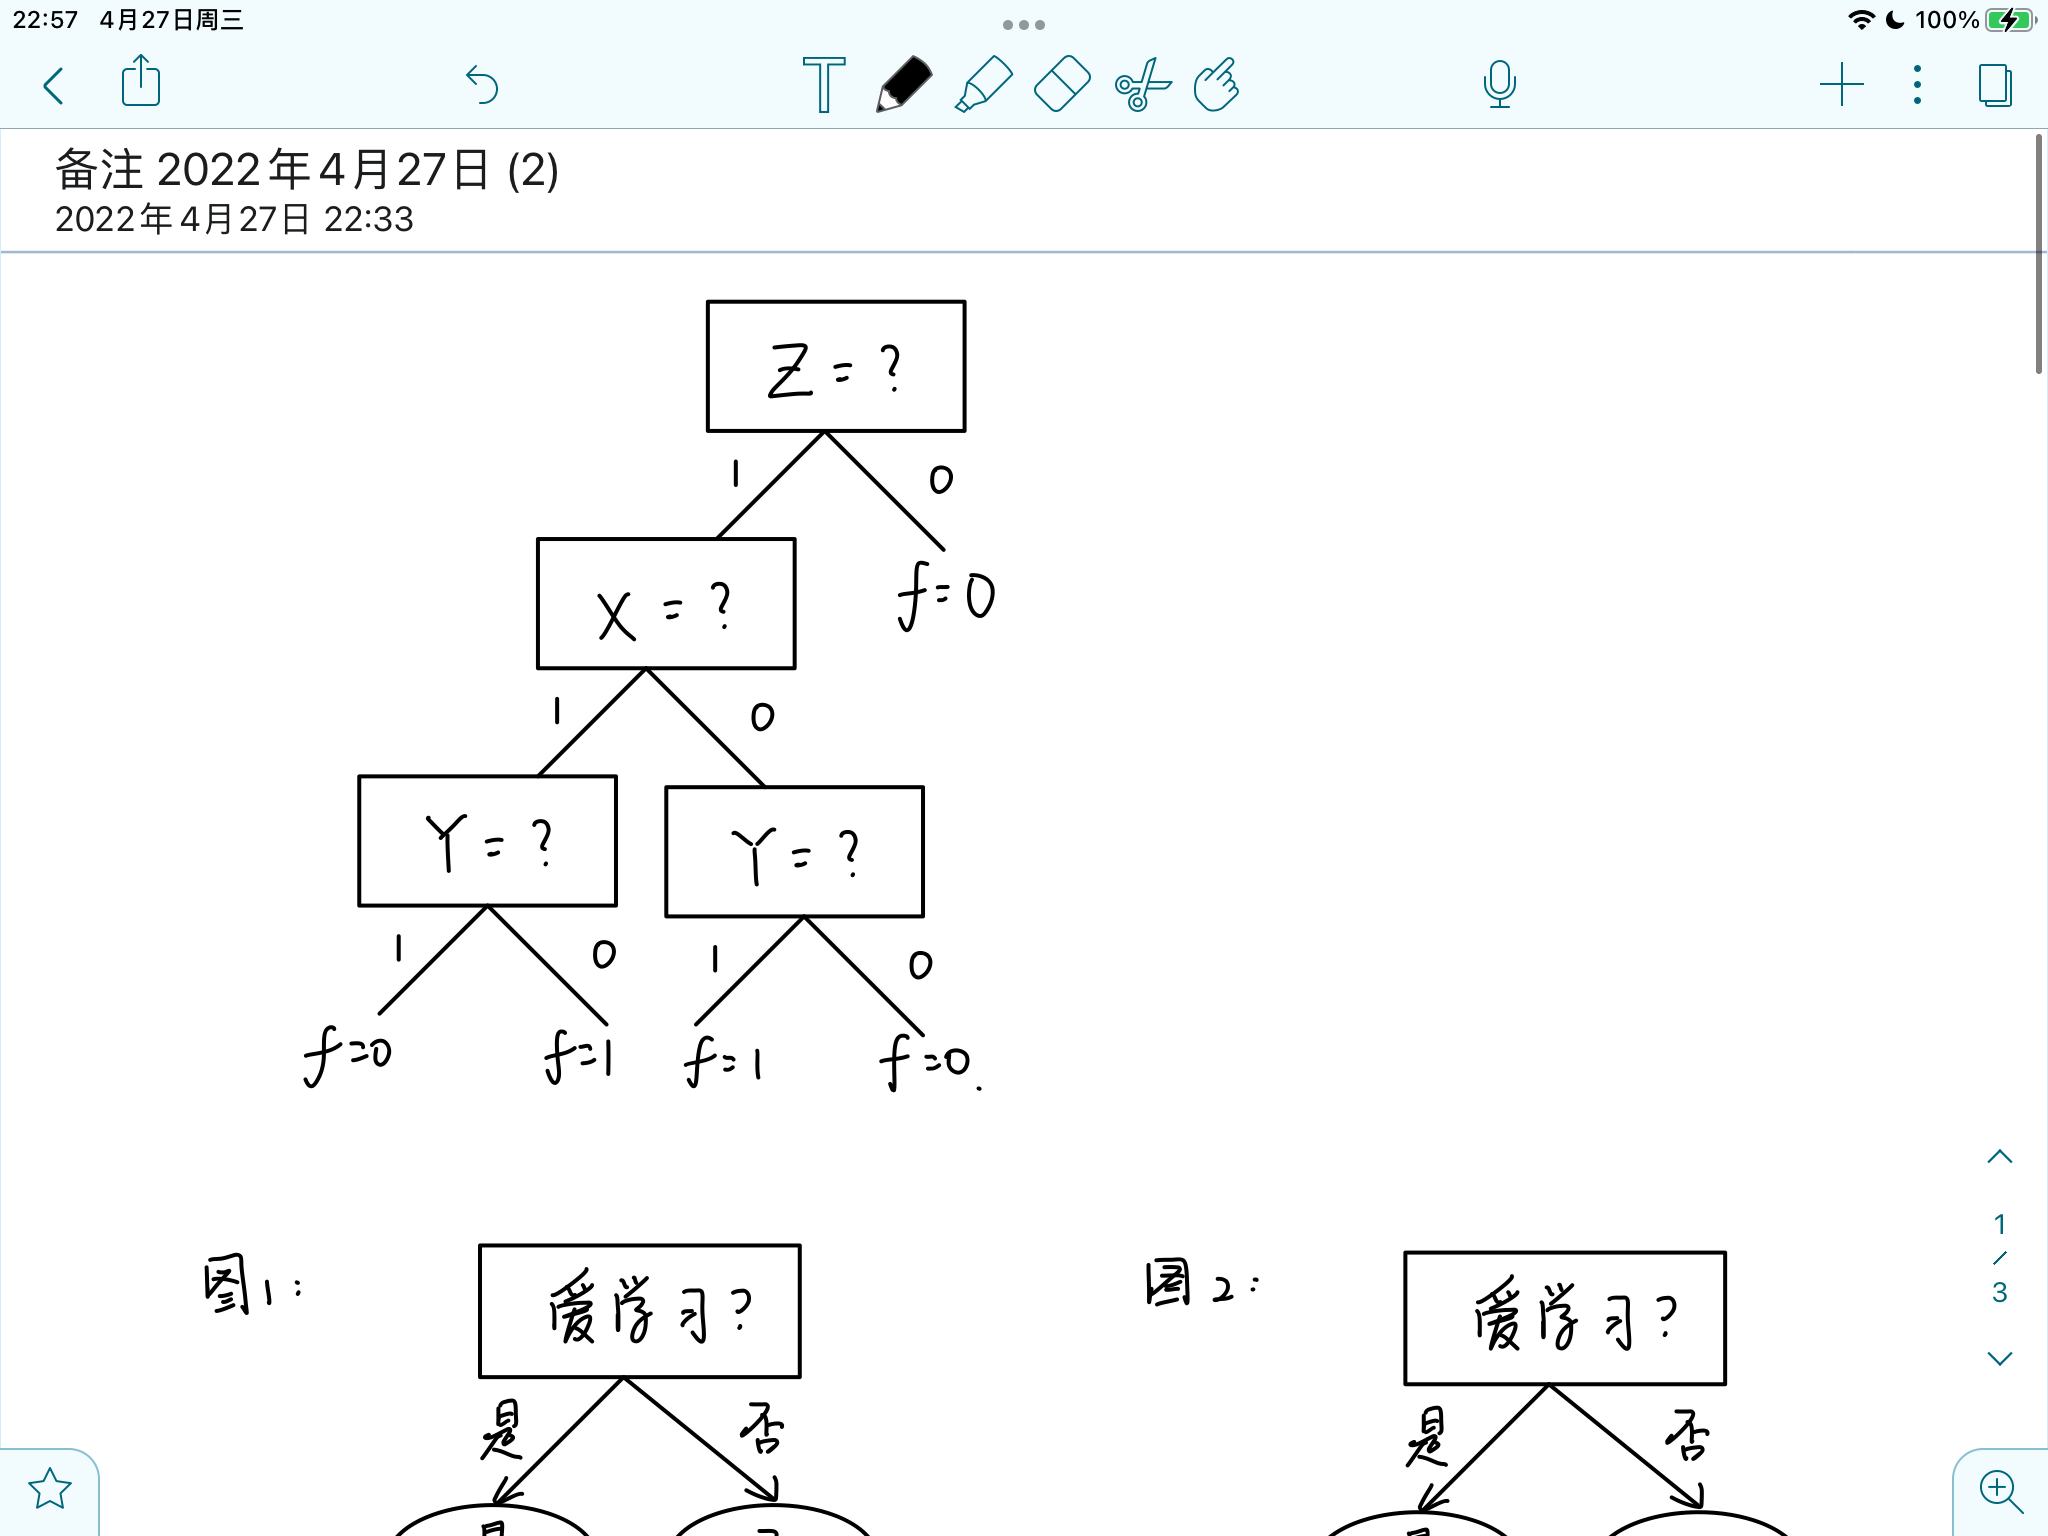
\includegraphics[width=9.5cm,height=9.5cm]{IMG_0162.png}
                      \caption{第2题图1}
                  \end{figure}
            \item 分别以X,Y,Z对D进行划分,得到的子集分别为$D^0,D^1$.\\
                  \begin{align*}
                      Gini(D,X) & =2\times (1-(\frac{1}{4} )^2-(\frac{3}{4})^2 )=0.375 \\
                      Gini(D,Y) & =2\times (1-(\frac{1}{4} )^2-(\frac{3}{4})^2 )=0.375 \\
                      Gini(D,Z) & =2\times (1-(\frac{0}{4} )^2-(\frac{4}{4})^2 )=0.25
                  \end{align*}
                  故以Z划分.然后分别以X,Y对{1,4,6,8}进行划分,得到的子集为$D_1^0,D_1^1$,此时X与Y的基尼指数相同,故以X划分,决策树如下:
                  \begin{figure}[H]
                      \centering
                      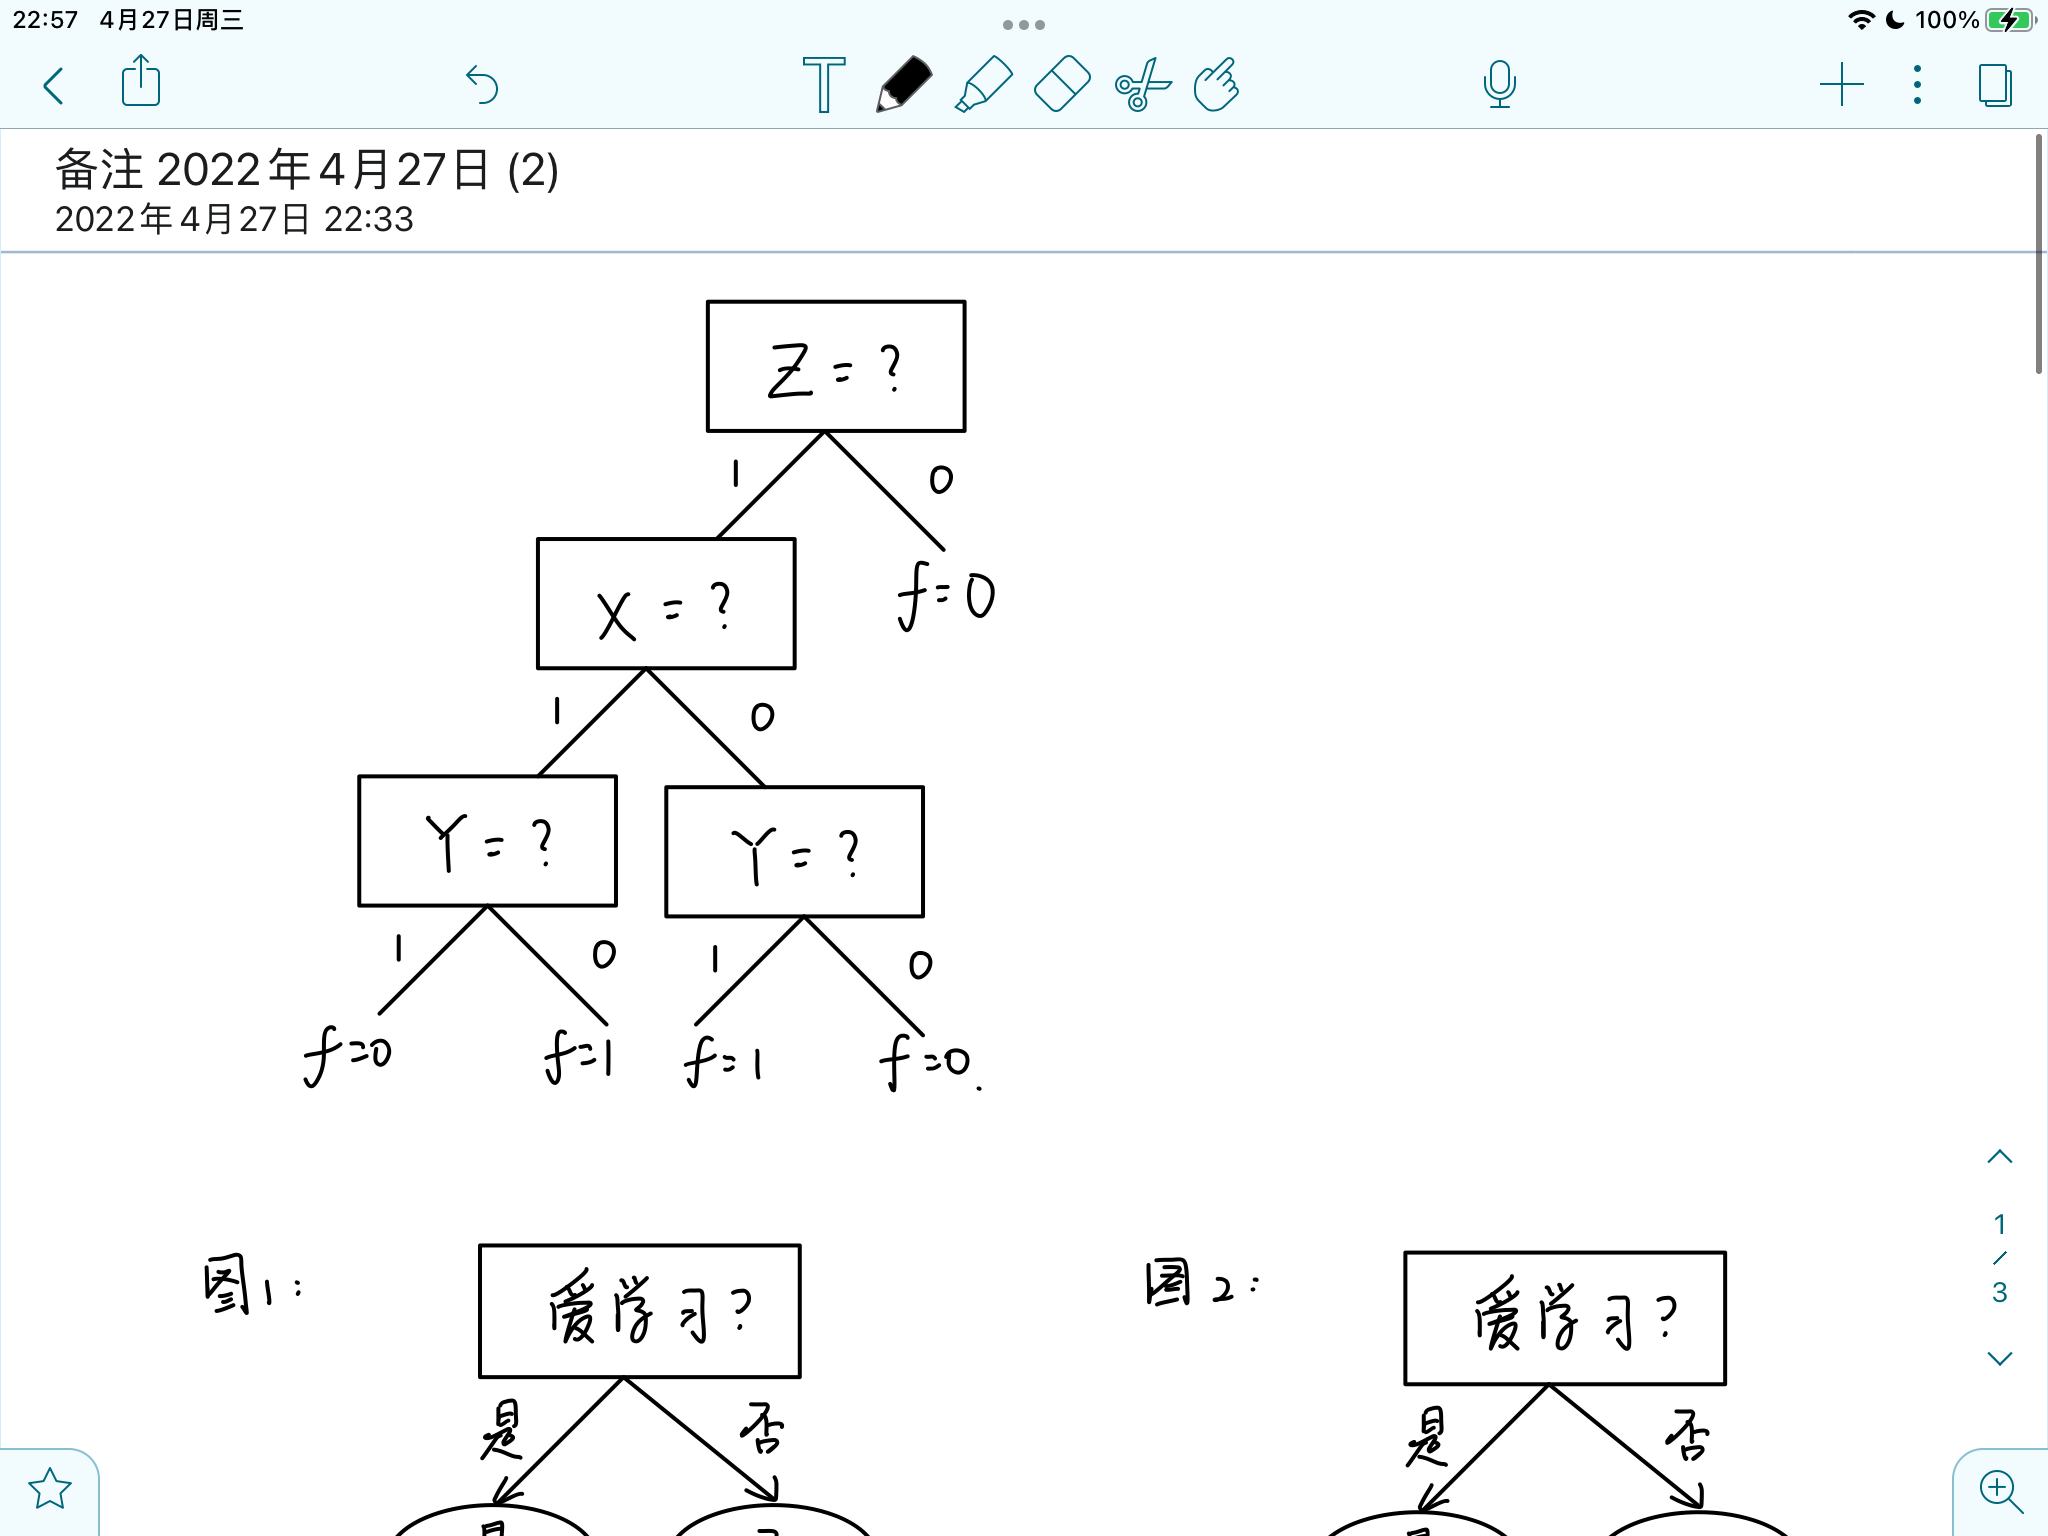
\includegraphics[width=9.5cm,height=9.5cm]{IMG_0162.png}
                      \caption{第2题图2}
                  \end{figure}
        \end{enumerate}
    \end{solution}


    \question [25] \textbf{决策树剪枝处理} \label{ch4_prob:prunning}

    教材4.3节介绍了决策树剪枝相关内容, 给定包含5个样例的人造数据集如表\ref{ch4_tab:artificial_training_dataset}所示, 其中“爱运动”、“爱学习”是属性, “成绩高”是标记. 验证集如表\ref{ch4_tab:artificial_testing_dataset}所示. 使用信息增益为划分准则产生如图\ref{ch4_fig:decision_tree_1}所示的两棵决策树. 请回答以下问题:
    \begin{table}[!htb]
        \caption{人造数据集}
        \begin{minipage}[t]{.48\linewidth}
            \subcaption{训练集}\label{ch4_tab:artificial_training_dataset}
            \centering
            \begin{tabular}{cccc}
                \hline 编号 & 爱运动 & 爱学习 & 成绩高 \\
                \hline 1    & 是     & 是     & 是     \\
                2           & 否     & 是     & 是     \\
                3           & 是     & 否     & 否     \\
                4           & 是     & 否     & 否     \\
                5           & 否     & 否     & 是     \\
                \hline
            \end{tabular}
        \end{minipage}%
        \begin{minipage}[t]{.48\linewidth}
            \centering
            \subcaption{验证集}\label{ch4_tab:artificial_testing_dataset}
            \begin{tabular}{cccc}
                \hline 编号 & 爱运动 & 爱学习 & 成绩高 \\
                \hline 6    & 是     & 是     & 是     \\
                7           & 否     & 是     & 否     \\
                8           & 是     & 否     & 否     \\
                9           & 否     & 否     & 否     \\
                \hline
            \end{tabular}
        \end{minipage}
    \end{table}
    \begin{figure}[ht]
        \centering
        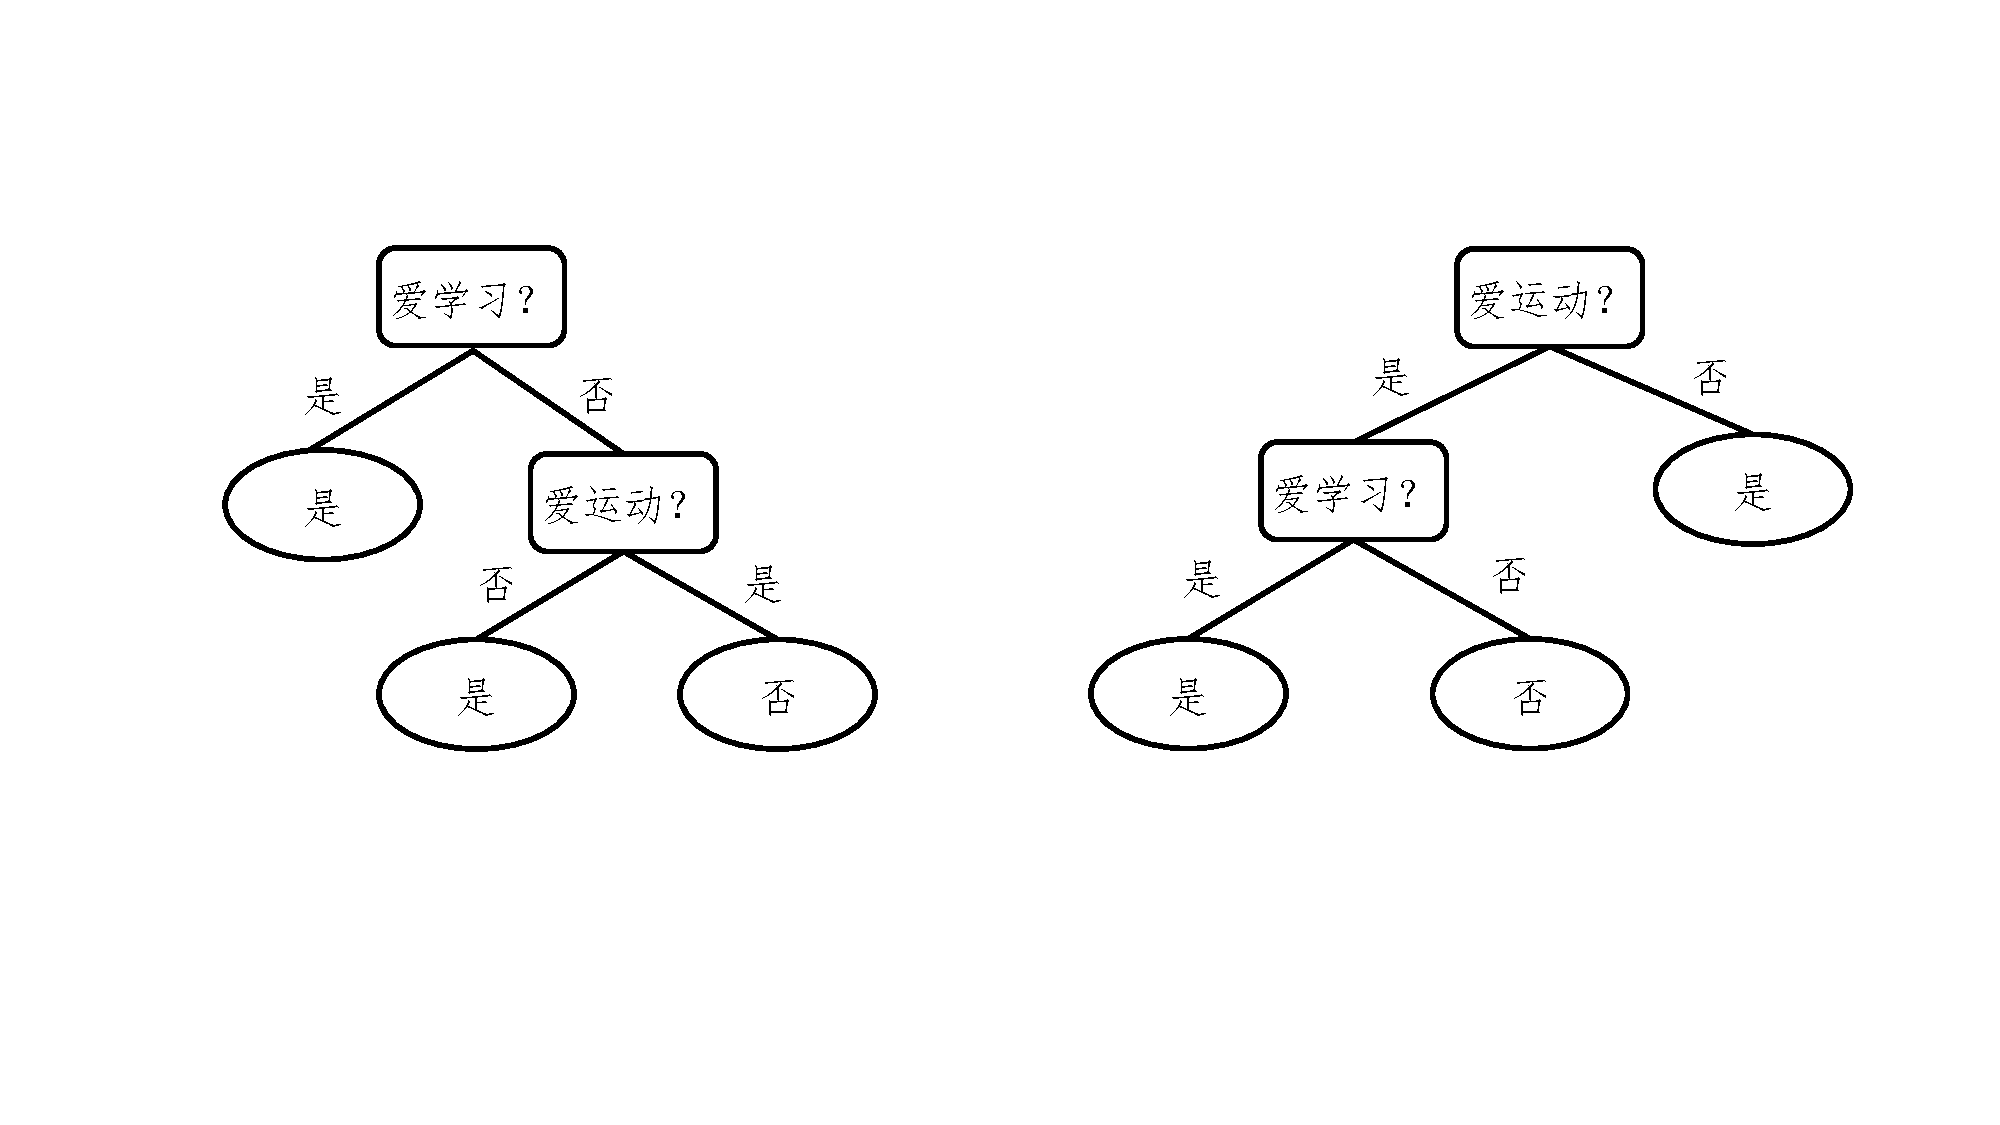
\includegraphics[width=0.8\textwidth]{figure/ch4_decision_tree_1.pdf}
        \caption{人造数据决策树结果}\label{ch4_fig:decision_tree_1}
    \end{figure}
    \begin{enumerate}
        \item
              请验证这两棵决策树的产生过程.
        \item
              对图\ref{ch4_fig:decision_tree_1}的结果基于该验证集进行预剪枝、后剪枝, 给出剪枝后的决策树.
        \item
              比较预剪枝、后剪枝的结果, 每种剪枝方法在训练集、验证集上的准确率分别为多少?哪种方法拟合能力较强?
    \end{enumerate}

    \begin{solution}
        \begin{enumerate}
            \item 对训练集,设爱运动为X,爱学习为Y,是为1,否为0.则有:
                  $\operatorname{Ent}(D)=-(\frac{3}{5} \log_2\frac{3}{5} +\frac{2}{5} \log_2\frac{2}{5})=0.971$\\
                  以爱学习划分时,有$Gain(D,Y)=-(\frac{2}{5} \log_2 \frac{2}{5} +\frac{3}{5} \log_2\frac{3}{5})+\frac{3}{5} (\frac{1}{3} \log_2\frac{1}{3} +\frac{2}{3} \log_2\frac{2}{3})$\\
                  以爱运动划分时,有$Gain(D,X)=-(\frac{2}{5} \log_2 \frac{2}{5} +\frac{3}{5} \log_2\frac{3}{5})+\frac{3}{5} (\frac{1}{3} \log_2\frac{1}{3} +\frac{2}{3} \log_2\frac{2}{3})$\\
                  因此其对根节点属性划分有两种选择,可以发现以这两种划分时得到的数据集是一样的,所以可以证明这两个决策树产生过程都是合理的.
            \item 以下四幅图分别表示左侧决策树预剪枝、后剪枝,右侧决策树预剪枝、后剪枝:
                  \begin{figure}[H]
                      \centering
                      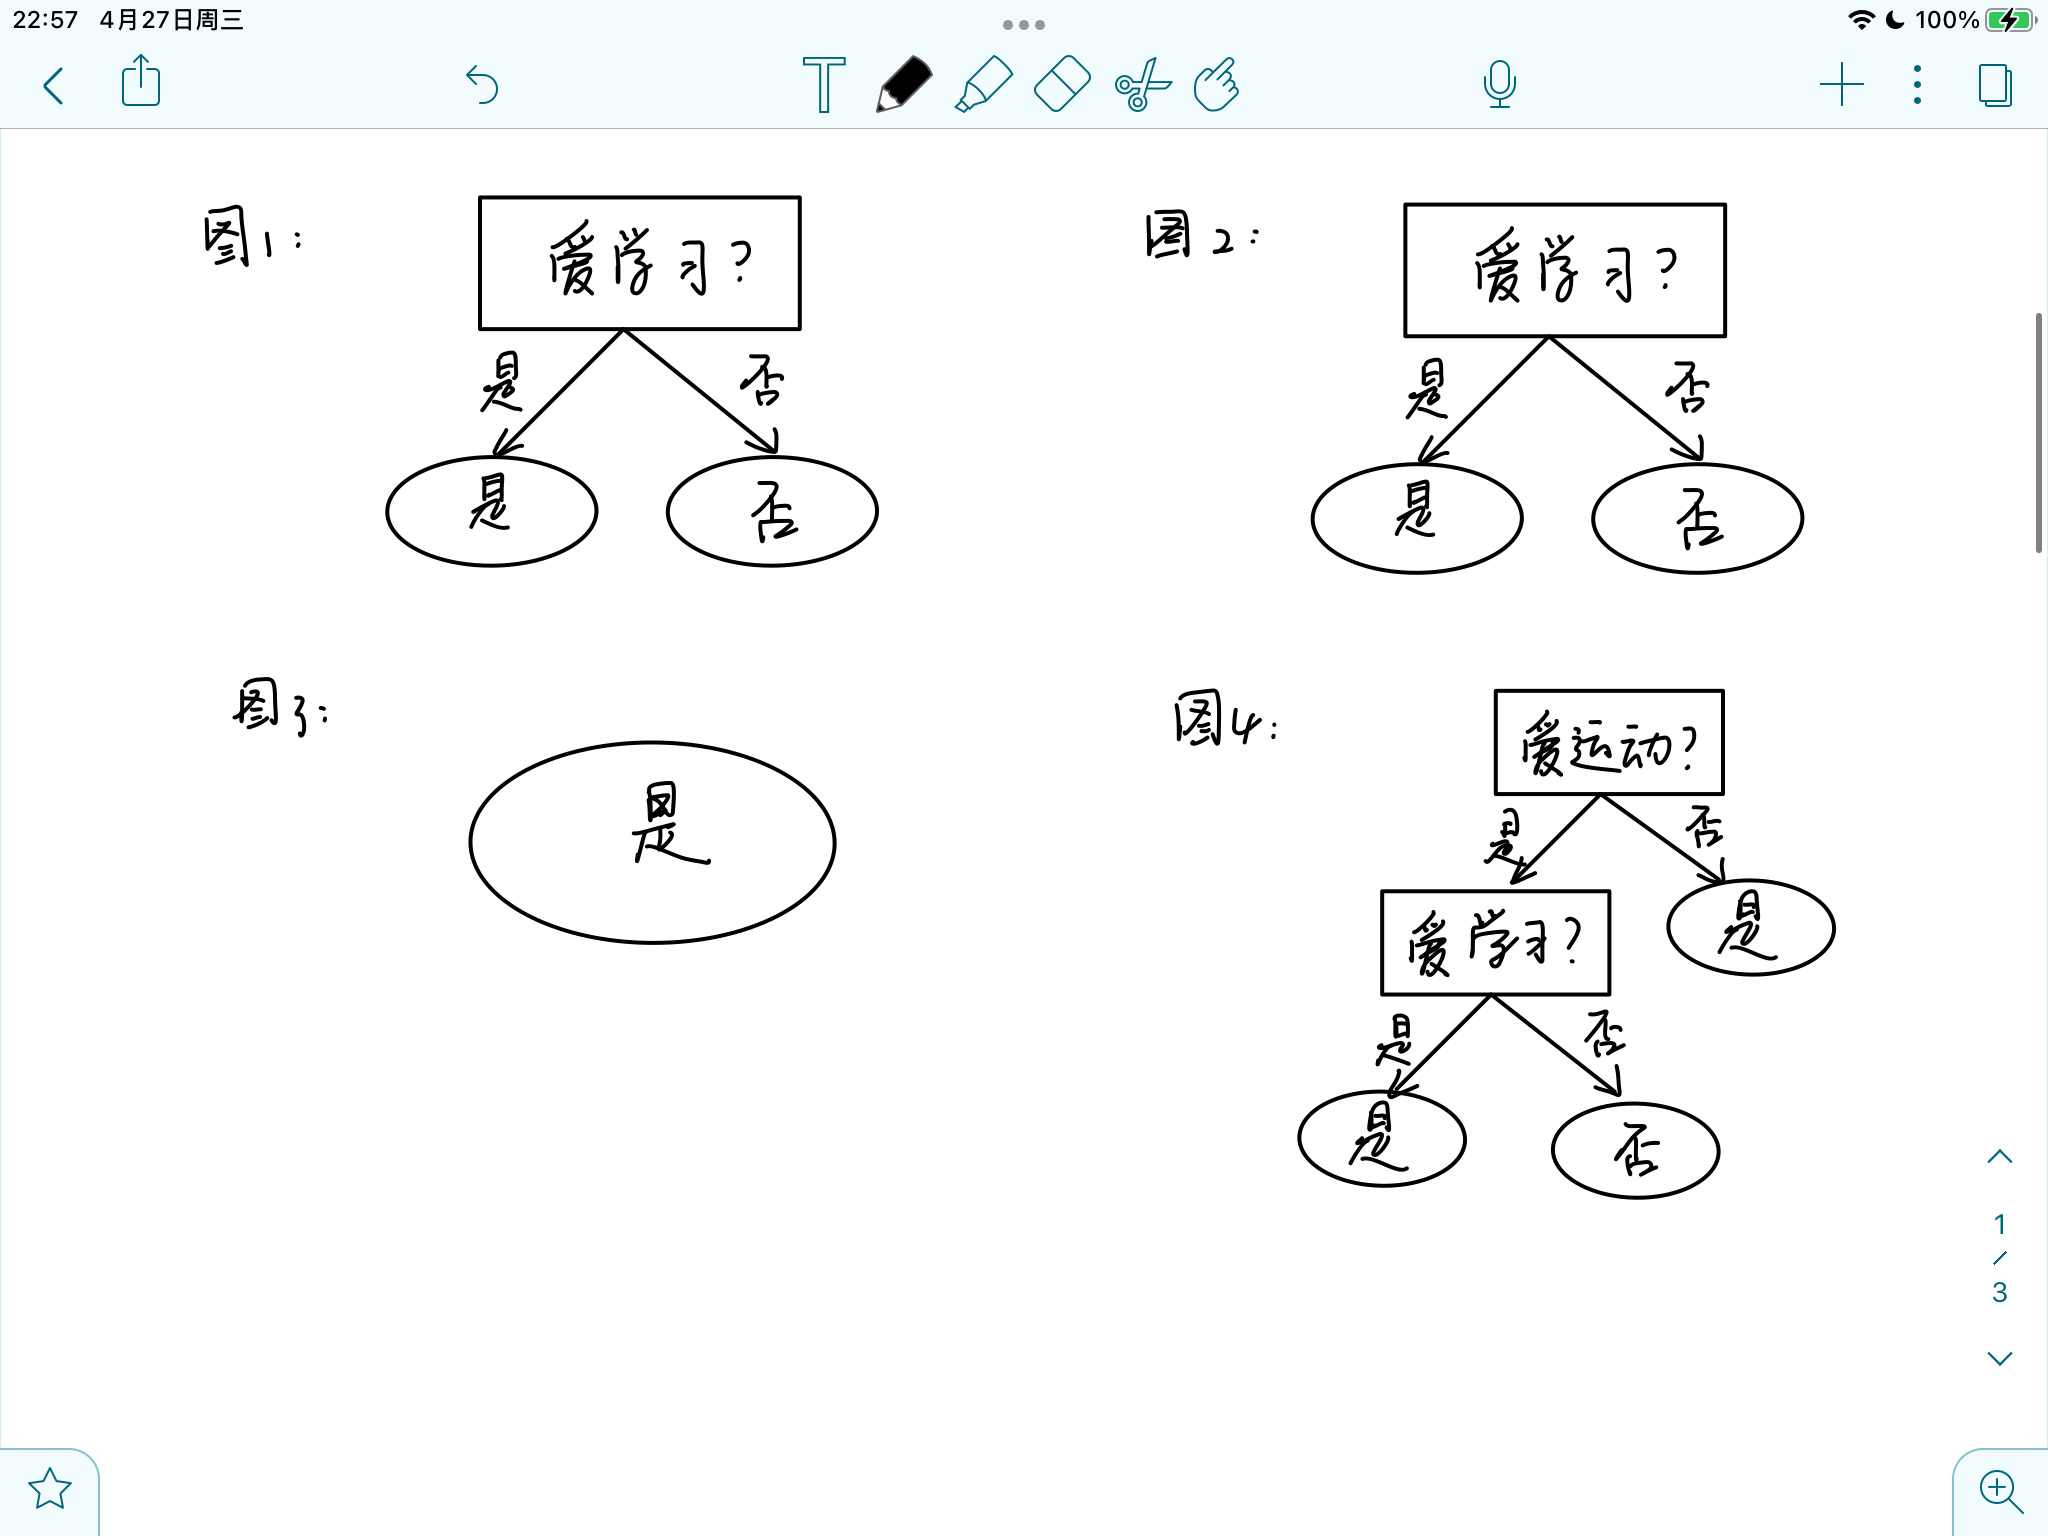
\includegraphics[height=9.5cm]{IMG_0163.png}
                      \caption{第3题图}
                  \end{figure}
            \item 决策树1:
                  \begin{tabular}{c|c|c}
                                    & 训练集 & 测试集 \\
                      \hline 预剪枝 & 0.8    & 0.75   \\
                      后剪枝        & 0.8    & 0.75   \\
                  \end{tabular}\\
                  决策树2:
                  \begin{tabular}{c|c|c}
                                    & 训练集 & 测试集 \\
                      \hline 预剪枝 & 0.6    & 0.25   \\
                      后剪枝        & 1.0    & 0.5    \\
                  \end{tabular}\\
                  因此可以发现后剪枝拟合能力强于预剪枝.
        \end{enumerate}
    \end{solution}

    \question [20] \textbf{连续与缺失值}



    \begin{enumerate}
        \item
              考虑如表~\ref{ch4_tab:continuous_small_dataset}所示数据集,仅包含一个连续属性,请给出将该属性“数字”作为划分标准时的决策树划分结果。
              \begin{table}[h]
                  \begin{center}
                      \begin{tabular}{cc}
                          \hline 属性 & 类别 \\
                          \hline 3    & 正   \\
                          4           & 负   \\
                          6           & 负   \\
                          9           & 正   \\
                          \hline
                      \end{tabular}
                      \caption{连续属性数据集}\label{ch4_tab:continuous_small_dataset}
                  \end{center}
              \end{table}
        \item 请阐述决策树如何处理训练时存在缺失值的情况,具体如下:考虑表~\ref{ch4_tab:bool_table}的数据集,如果发生部分缺失,变成如表~\ref{ch4_tab:missing_dataset}所示数据集(假设$X, Y, Z$只有0和1两种取值).
              \begin{table}[ht]
                  \centering
                  \caption{缺失数据集}\label{ch4_tab:missing_dataset}
                  \begin{tabular}{ccc|c}
                      \hline X & Y & Z & $f$ \\
                      \hline
                      1        & 0 & - & 1   \\
                      -        & 1 & 0 & 0   \\
                      0        & - & 0 & 0   \\
                      0        & 1 & 1 & 1   \\
                      -        & 1 & 0 & 0   \\
                      0        & 0 & - & 0   \\
                      1        & - & 0 & 0   \\
                      1        & 1 & 1 & 0   \\
                      \hline
                  \end{tabular}
              \end{table}
              在这种情况下,请考虑如何处理数据中的缺失值,并结合问题~\ref{ch4_prob:get_tree}第1小问的答案进行对比,论述方法的特点以及是否有局限性。
        \item 请阐述决策树如何处理测试时存在缺失值的情况,具体如下:对于问题~\ref{ch4_prob:prunning}训练出的决策树,考虑表~\ref{ch4_tab:artificial_testing_dataset2}所示的含有缺失值的测试集,输出其标签,并论述方法的特点以及是否有局限性。
              \begin{table}[ht]
                  \centering
                  \caption{缺失数据集}\label{ch4_tab:artificial_testing_dataset2}
                  \begin{tabular}{cccc}
                      \hline 编号 & 爱运动 & 爱学习 & 成绩高 \\
                      \hline 6    & 是     & -      &        \\
                      7           & -      & 是     &        \\
                      8           & 否     & -      &        \\
                      9           & -      & 否     &        \\
                      \hline
                  \end{tabular}
              \end{table}

    \end{enumerate}
    \begin{solution}
        \begin{enumerate}
            \item 	    进行连续值处理,可以得到划分点集合$T_a=\{3.5,5,7.5\}$

                  属性信息增益计算结果如下:
                  \begin{align*}
                      Gain(D,a,3.5)= & -(\frac{1}{2}log_2\frac{1}{2}+\frac{1}{2}log_2\frac{1}{2})+ \\&\frac{3}{4}(\frac{1}{3}log_2\frac{1}{3}+\frac{2}{3}log_2\frac{2}{3})]=0.311\\
                      Gain(D,a,5)=   & -(\frac{1}{2}log_2\frac{1}{2}+\frac{1}{2}log_2\frac{1}{2})+ \\&2\times \frac{1}{2} (\frac{1}{2}log_2\frac{1}{2}+\frac{1}{2}log_2\frac{1}{2})]=0\\
                      Gain(D,a,7.5)= & -(\frac{1}{2}log_2\frac{1}{2}+\frac{1}{2}log_2\frac{1}{2})+ \\&\frac{3}{4}(\frac{1}{3}log_2\frac{1}{3}+\frac{2}{3}log_2\frac{2}{3})]=0.311
                  \end{align*}

                  故可以选择3.5和7.5两个划分点,当选取3.5为划分点时得到两个分支:$D^0=\{3\},D^1=\{4,6,9\}$

                  选取7.5为划分点时得到两个分支:$D^0=\{3,4,6\},D^1=\{9\}$
            \item 计算信息增益可以得到:
                  \begin{align*}
                      X:\operatorname{Ent}(\tilde{D})   & =-(\frac{1}{3} \log_2\frac{1}{3} +\frac{2}{3} \log_2\frac{2}{3}) =0.918                                                            \\
                      Gain(D,X)                         & =\frac{3}{4} \times (0.918-[\frac{3}{6} (-\frac{1}{3} \log_2\frac{1}{3} -\frac{2}{3} \log_2\frac{2}{3})+                           \\&\frac{3}{6} (-\frac{1}{3} \log_2\frac{1}{3} -\frac{2}{3}\log_2\frac{2}{3})])=0 \\
                      Y:\operatorname{Ent}(\tilde{D})   & =-(\frac{1}{3} \log_2\frac{1}{3} +\frac{2}{3} \log_2\frac{2}{3}) =0.918                                                            \\Gain(D,Y)&=\frac{3}{4} \times (0.918-[\frac{2}{6} (-\frac{1}{2} \log_2\frac{1}{2} -\frac{1}{2} \log_2\frac{1}{2})\\&+\frac{4}{6} (-\frac{1}{4} \log_2\frac{1}{4} -\frac{3}{4}\log_2\frac{3}{4})])=0.0329\\
                      Z:  \operatorname{Ent}(\tilde{D}) & =-(\frac{1}{6} \log_2\frac{1}{6} +\frac{5}{6} \log_2\frac{5}{6})=0.650                                                             \\
                      Gain(D,Z)                         & =\frac{3}{4} \times (0.650-[\frac{4}{6} (-0-0)+\frac{2}{6} (\frac{1}{2} \log_2\frac{1}{2} -\frac{1}{2} \log_2\frac{1}{2} )])=0.238
                  \end{align*}
                  所以第一个划分属性为Z,得到两个分支,其中编号为2,3,5,7的进入"Z=0"分支,编号为4,8的进入"Z=1"分支,编号为1,6的同事进入两个分支,在两个分支的权重分别为$\frac{2}{3},\frac{1}{3} $\\
                  对于分支"Z=0"计算信息增益有:
                  \begin{align*}
                      Gain(D^0,X) & =\frac{2}{3} (\operatorname{Ent}(\tilde{D}^0)+\frac{1}{2} (\frac{1}{2} \log_2 \frac{1}{2}+\frac{1}{2} \log_2 \frac{1}{2})) \\
                      Gain(D^0,Y) & =\frac{2}{3} (\operatorname{Ent}(\tilde{D}^0)+\frac{2}{5} (\frac{1}{2} \log_2 \frac{1}{2}+\frac{1}{2} \log_2 \frac{1}{2}))
                  \end{align*}
                  所以由于$Gain(D^0,Y)$大,即此时第二个划分属性为Y,同理对另一个分支,此时第二个划分属性为X.决策树如下:
                  \begin{figure}[H]
                      \centering
                      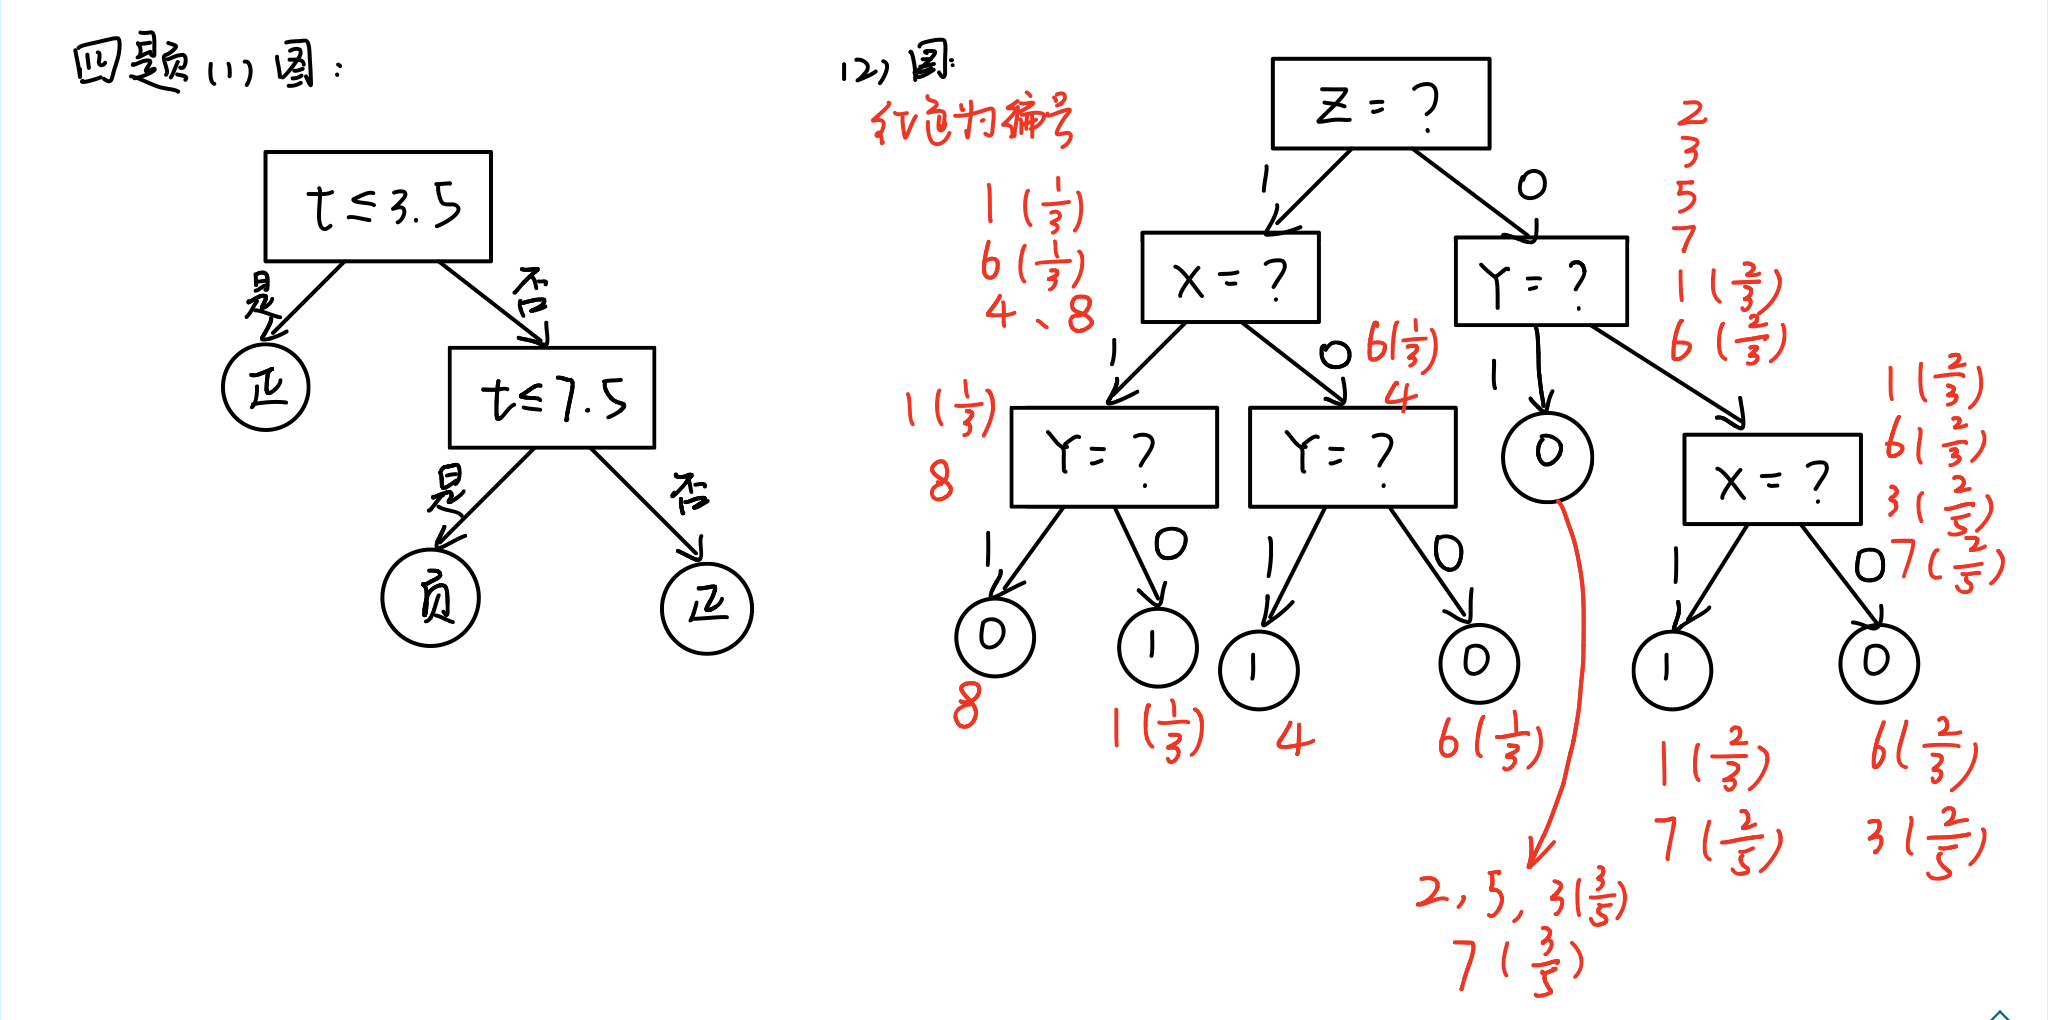
\includegraphics[width=14.5cm,height=9.5cm]{IMG_0161.png}
                      \caption{第4题图}
                  \end{figure}

                  由此可见,大部分的样本依旧分类正确,仅有样本1,3,6,7号以不同的概率进入不同节点,其中1,3,6号样本所有概率都取值为0,仅有7号样本有$\frac{2}{5} $的概率分类错误.所以该方法具有较高泛化能力,表现较好.
            \item 当测试时出现缺失值时,就同时探查所有的可能分支,计算每个类别的概率,取概率最大的类别赋值给该样本.对于第三题的验证集若部分属性缺失,则输出如下:
                  \begin{center}
                      \begin{tabular}{c|ccc}
                          \hline   & 爱运动 & 爱学习 & 成绩高       \\
                          \hline 6 & 是     & -      & 一半是一半否 \\
                          7        & -      & 否     & 是           \\
                          8        & 否     & -      & 是           \\
                          9        & -      & 否     & 一半是一半否 \\
                          \hline
                      \end{tabular}

                      \begin{tabular}{c|ccc}
                          \hline   & 爱运动 & 爱学习 & 成绩高       \\
                          \hline 6 & 是     & -      & 一半是一半否 \\
                          7        & -      & 否     & 是           \\
                          8        & 否     & -      & 是           \\
                          9        & -      & 否     & 一半是一半否 \\
                          \hline
                      \end{tabular}
                  \end{center}
        \end{enumerate}
    \end{solution}


    \question [20] \textbf{多变量决策树}

    考虑如下包含10个样本的数据集, 每一列表示一个样本, 每个样本具有二个属性, 即$\vx_i = (x_{i1};\; x_{i2})$.
    \begin{table}[ht]
        \begin{center}
            \begin{tabular}{ccccccccccc}
                \hline 编号  & 1  & 2  & 3  & 4  & 5  & 6   & 7  & 8  & 9  & 10 \\
                \hline $A_1$ & 24 & 53 & 23 & 25 & 32 & 52  & 22 & 43 & 52 & 48 \\
                $A_2$        & 40 & 52 & 25 & 77 & 48 & 110 & 38 & 44 & 27 & 65 \\
                \hline 标记  & 1  & 0  & 0  & 1  & 1  & 1   & 1  & 0  & 0  & 1  \\
                \hline
            \end{tabular}
        \end{center}
    \end{table}
    \begin{enumerate}
        \item 计算根结点的熵;
        \item 构建分类决策树, 描述分类规则和分类误差;
        \item 根据 $\alpha x_{1}+\beta x_{2}-1$,  构建多变量决策树,描述树的深度以及 $\alpha$ 和 $\beta$ 的值.
    \end{enumerate}
    \begin{solution}
        \begin{enumerate}
            \item
                  \begin{align*}
                      \operatorname{Ent}(Root)=-(\frac{2}{5} \log_2 \frac{2}{5}+\frac{3}{5} \log_2\frac{3}{5})=0.971.
                  \end{align*}
            \item 对$A_1,A_2$两个特征进行离散处理,并根据基尼系数作为划分属性的评价指标.根据其基尼系数值得到最小的划分标准($A_2$)32.5作为第一轮决策树划分标准,分类之后,第二轮中最小的划分标准($A_1$)52.5作为第二轮决策树划分标准,依次类推,每次删除成功分类的点并递归进行该过程,直到可以将所有的特征都分类完成,决策树如下:
            \item \begin{figure}[H]
                      \centering
                      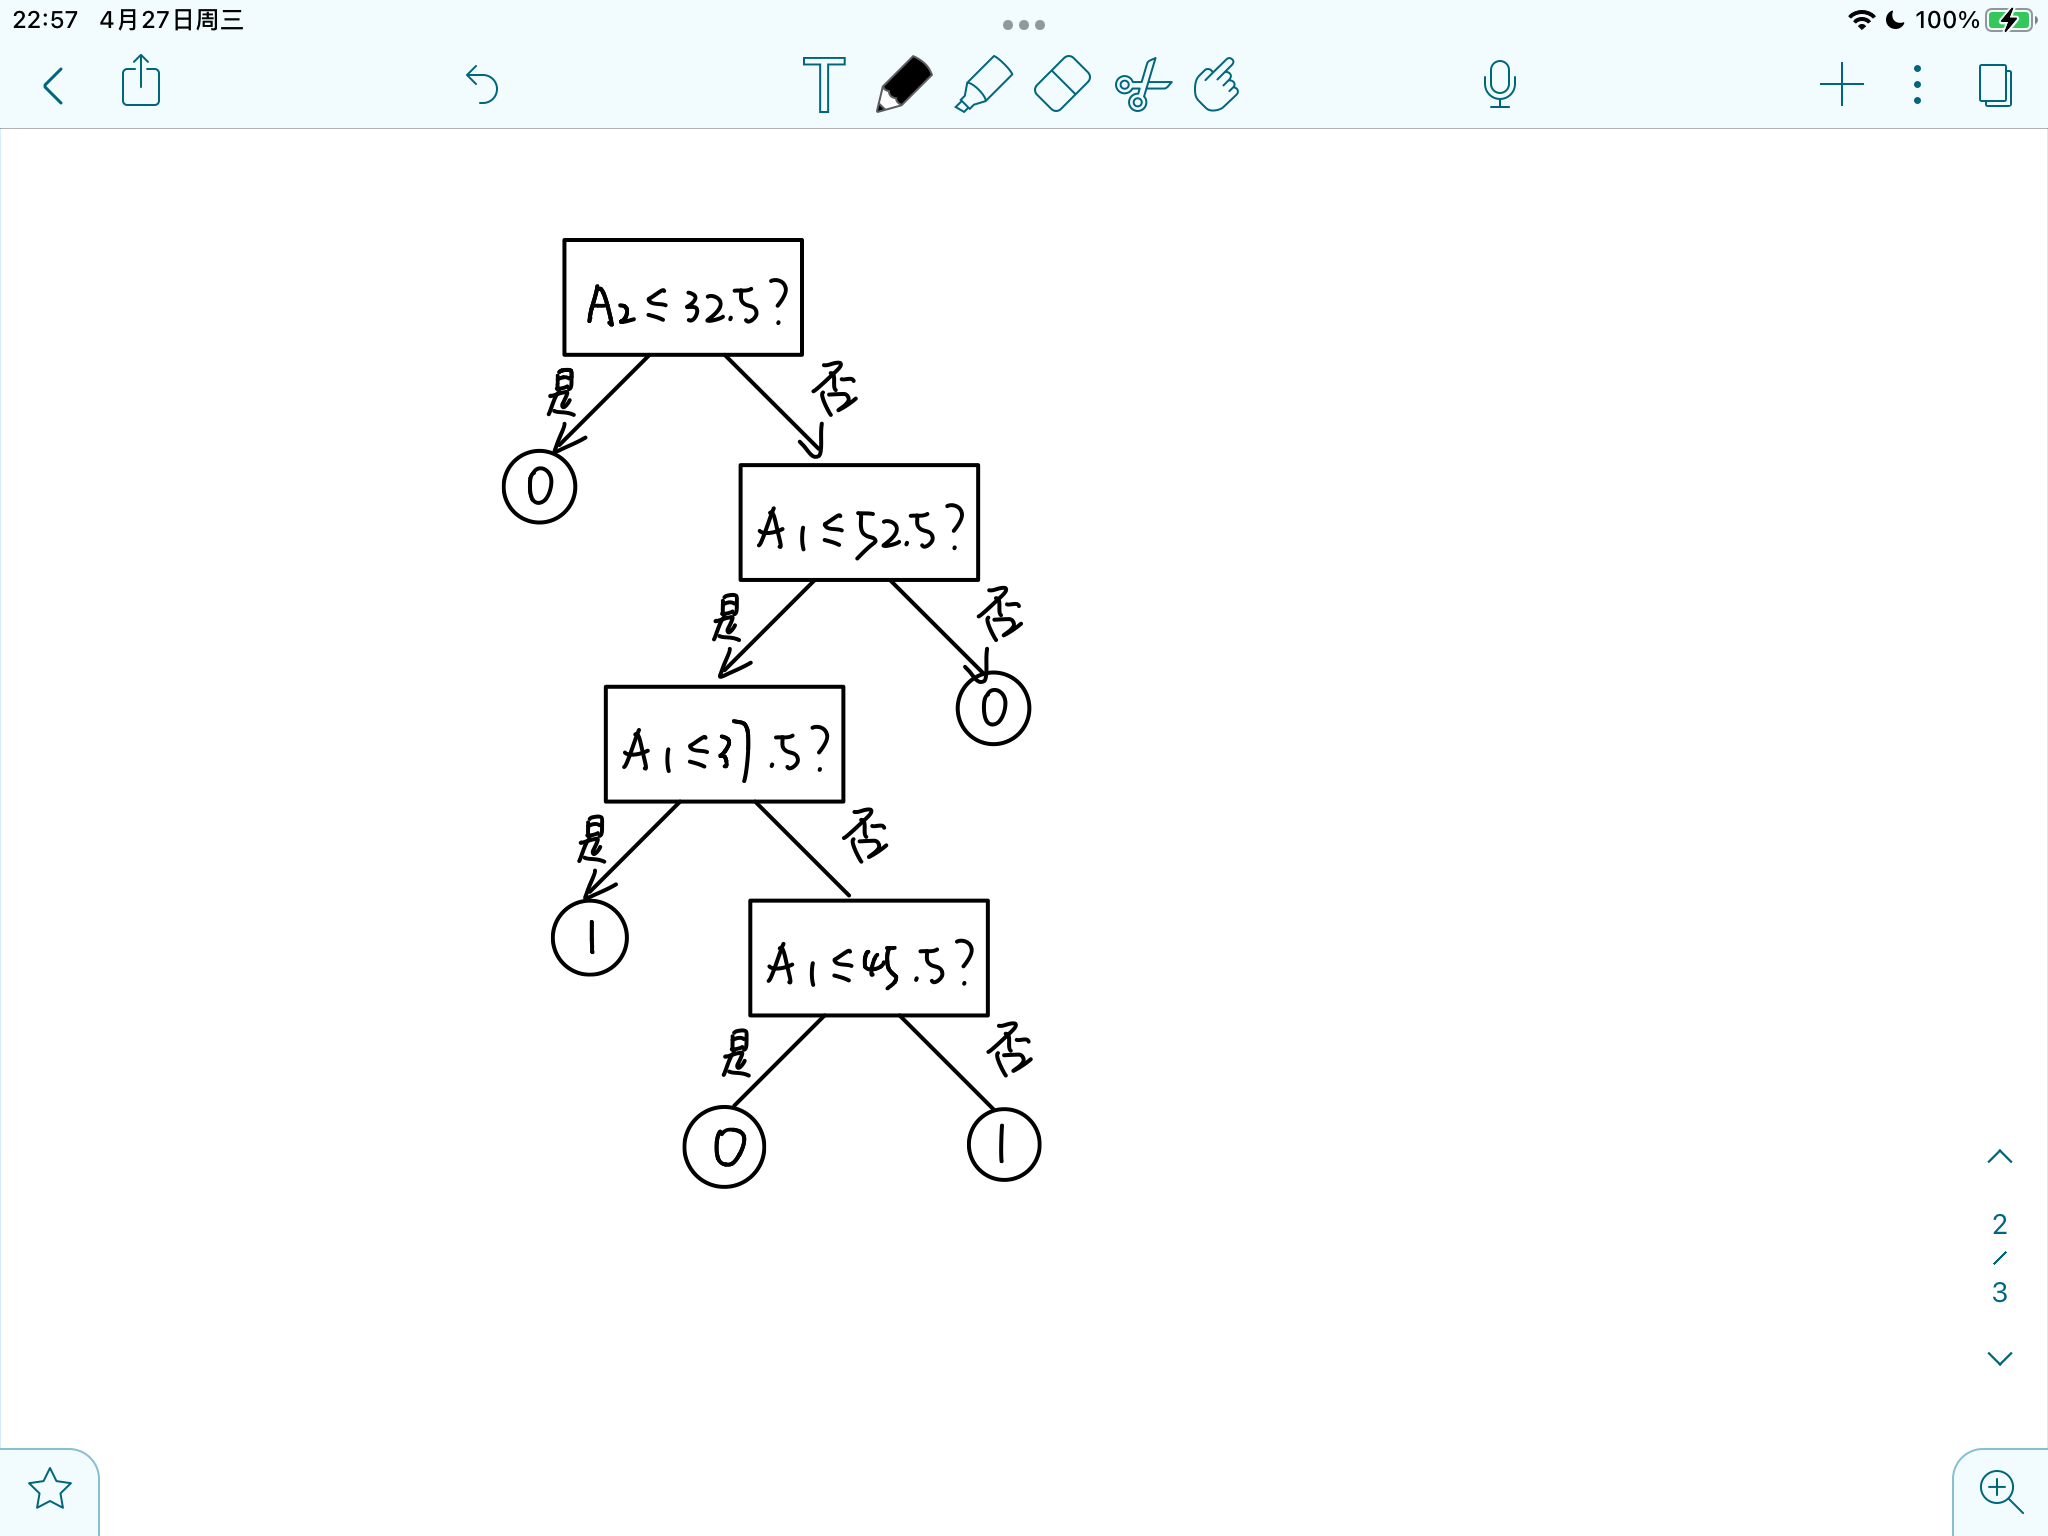
\includegraphics[width=14.5cm,height=9.5cm]{IMG_0159.png}
                      \caption{第5题图}
                  \end{figure}
        \end{enumerate}
    \end{solution}

\end{questions}


\end{document}